\documentclass[mathNotesPreamble]{subfiles}
\begin{document}
\relscale{1.4} %TODO
\section{13.6: Cylinders and Quadric Surfaces}
  \begin{defn*}[Trace]
    A \textbf{trace} of a surface is the set of points at which the surface intersects a plane that is parallel to one of the coordinate planes. The traces in the coordinate planes are called the \textbf{$xy$-trace}, the \textbf{$yz$-trace}, and the \textbf{$xz$-trace} (Figure 13.80).
  \end{defn*}
  \begin{center}
    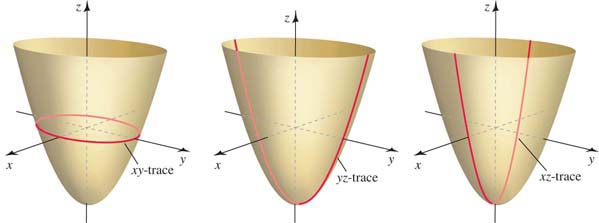
\includegraphics[width=0.75\linewidth]{images/briggs_13_06/fig13_80}
  \end{center}
  \pagebreak
  
  \begin{center}
  %https://tex.stackexchange.com/questions/337570/tabularx-with-different-column-widths
    \renewcommand{\tabularxcolumn}[1]{m{#1}} %sets columns to vertically centered
    \relscale{0.775}
    \begin{tabularx}{\linewidth}{@{}
      >{\hsize=0.25\hsize}X@{\hspace*{20pt}}
      >{\hsize=0.45\hsize}X
      >{\hsize=0.725\hsize}X
      >{\hsize=0.4\hsize}Y@{}}\toprule
      \textbf{Name}& 
      \textbf{Standard Equation}& 
      \multicolumn{1}{c}{\textbf{Features}}&
      \textbf{Graph}\\\midrule
      %
      Ellipsoid& 
      $\displaystyle \frac{x^2}{a^2}+\frac{y^2}{b^2}+\frac{z^2}{c^2}=1$& 
      All traces are ellipses.& 
      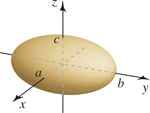
\includegraphics[width=0.25\linewidth]{images/briggs_13_06/tab13_1_fig1}\\
      %
      Elliptic paraboloid& 
      $\displaystyle z=\frac{x^2}{a^2}+\frac{y^2}{b^2}$& 
      Traces with $z=z_0>0$ are ellipses. Traces with $x=x_0$ or $y=y_0$ are parabolas.& 
      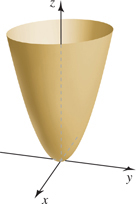
\includegraphics[width=0.25\linewidth]{images/briggs_13_06/tab13_1_fig2}\\
      %
      Hyperboloid of one sheet& 
      $\displaystyle \frac{x^2}{a^2}+\frac{y^2}{b^2}-\frac{z^2}{c^2}=1$& 
      Traces with $z=z_0$ are ellipses for all $z_0$. Traces with $x=x_0$ or $y=y_0$ are hyperbolas.& 
      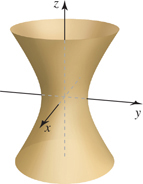
\includegraphics[width=0.25\linewidth]{images/briggs_13_06/tab13_1_fig3}\\
      %
      Hyperboloid of two sheets& 
      $\displaystyle -\frac{x^2}{a^2}-\frac{y^2}{b^2}+\frac{z^2}{c^2}=1$&
      Traces with $z=z_0$ with $\abs{z_0}>\abs{c}$ are ellipses. Traces with $x=x_0$ and $y=y_0$ are hyperbolas.& 
      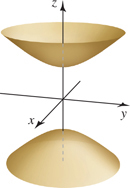
\includegraphics[width=0.25\linewidth]{images/briggs_13_06/tab13_1_fig4}\\
      %
      Elliptic cone& 
      $\displaystyle \frac{x^2}{a^2}+\frac{y^2}{b^2}=\frac{z^2}{c^2}$& 
      Traces with $z=z_0\neq0$ are ellipses. Traces with $x=x_0$ or $y=y_0$ are hyperbolas or intersecting lines.& 
      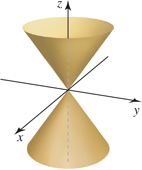
\includegraphics[width=0.25\linewidth]{images/briggs_13_06/tab13_1_fig5}\\
      %
      Hyperbolic paraboloid& 
      $\displaystyle z=\frac{x^2}{a^2}-\frac{y^2}{b^2}$& 
      Traces with $z=z_0\neq0$ are hyperbolas. Traces with $x=x_0$ or $y=y_0$ are parabolas.& 
      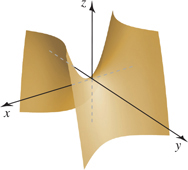
\includegraphics[width=0.3\linewidth]{images/briggs_13_06/tab13_1_fig6}\\
      %
      \bottomrule
    \end{tabularx}
  \end{center}
  \pagebreak
  
\end{document}